% Auto-generated from backend/data/app.db: per-slot share of quality-weighted,
% pose-attributed exposure, weighted-averaged across eight full-highlight
% analyses (M01-M04, M06-M08, M11; M05 excluded after attribution audit).
% Regenerate with scratchpad gen_paper_figs.py.
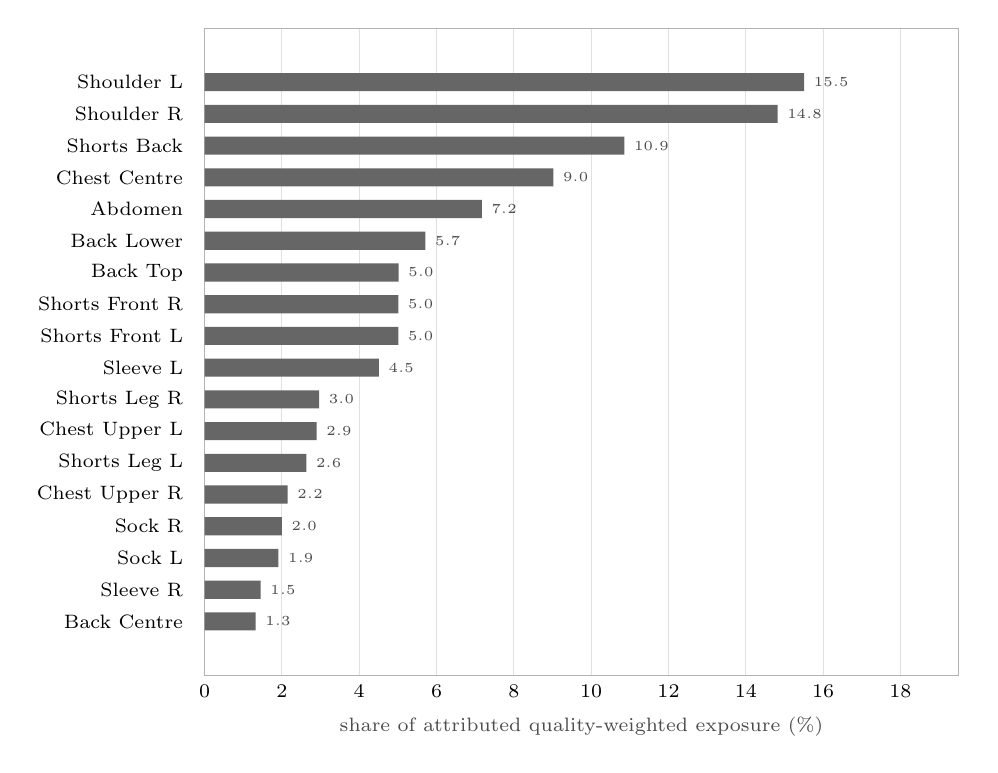
\begin{tikzpicture}
\begin{axis}[
  xbar, width=0.92\linewidth, height=98mm,
  xmin=0, xmax=19.5,
  symbolic y coords={Back Centre,Sleeve R,Sock L,Sock R,Chest Upper R,Shorts Leg L,Chest Upper L,Shorts Leg R,Sleeve L,Shorts Front L,Shorts Front R,Back Top,Back Lower,Abdomen,Chest Centre,Shorts Back,Shoulder R,Shoulder L},
  ytick=data, y dir=normal,
  bar width=2.3mm,
  axis line style={black!30},
  xmajorgrids, grid style={black!12},
  xlabel={share of attributed quality-weighted exposure (\%)},
  xlabel style={font=\scriptsize, color=black!70},
  tick label style={font=\scriptsize},
  ytick style={draw=none}, xtick style={draw=none},
  nodes near coords, nodes near coords align={horizontal},
  every node near coord/.append style={font=\tiny, color=black!70,
    /pgf/number format/fixed, /pgf/number format/fixed zerofill,
    /pgf/number format/precision=1},
]
\addplot[xbar, fill=black!60, draw=none] coordinates {
  (1.32,{Back Centre})
  (1.45,{Sleeve R})
  (1.91,{Sock L})
  (2.00,{Sock R})
  (2.15,{Chest Upper R})
  (2.63,{Shorts Leg L})
  (2.90,{Chest Upper L})
  (2.96,{Shorts Leg R})
  (4.51,{Sleeve L})
  (5.01,{Shorts Front L})
  (5.01,{Shorts Front R})
  (5.02,{Back Top})
  (5.71,{Back Lower})
  (7.17,{Abdomen})
  (9.02,{Chest Centre})
  (10.86,{Shorts Back})
  (14.82,{Shoulder R})
  (15.51,{Shoulder L})
};
\end{axis}
\end{tikzpicture}
